\documentclass[]{article}
\usepackage{lmodern}
\usepackage{amssymb,amsmath}
\usepackage{ifxetex,ifluatex}
\usepackage{fixltx2e} % provides \textsubscript
\ifnum 0\ifxetex 1\fi\ifluatex 1\fi=0 % if pdftex
  \usepackage[T1]{fontenc}
  \usepackage[utf8]{inputenc}
\else % if luatex or xelatex
  \ifxetex
    \usepackage{mathspec}
    \usepackage{xltxtra,xunicode}
  \else
    \usepackage{fontspec}
  \fi
  \defaultfontfeatures{Mapping=tex-text,Scale=MatchLowercase}
  \newcommand{\euro}{€}
\fi
% use upquote if available, for straight quotes in verbatim environments
\IfFileExists{upquote.sty}{\usepackage{upquote}}{}
% use microtype if available
\IfFileExists{microtype.sty}{\usepackage{microtype}}{}
\usepackage[margin=1in]{geometry}
\usepackage{color}
\usepackage{fancyvrb}
\newcommand{\VerbBar}{|}
\newcommand{\VERB}{\Verb[commandchars=\\\{\}]}
\DefineVerbatimEnvironment{Highlighting}{Verbatim}{commandchars=\\\{\}}
% Add ',fontsize=\small' for more characters per line
\newenvironment{Shaded}{}{}
\newcommand{\KeywordTok}[1]{\textcolor[rgb]{0.00,0.44,0.13}{\textbf{{#1}}}}
\newcommand{\DataTypeTok}[1]{\textcolor[rgb]{0.56,0.13,0.00}{{#1}}}
\newcommand{\DecValTok}[1]{\textcolor[rgb]{0.25,0.63,0.44}{{#1}}}
\newcommand{\BaseNTok}[1]{\textcolor[rgb]{0.25,0.63,0.44}{{#1}}}
\newcommand{\FloatTok}[1]{\textcolor[rgb]{0.25,0.63,0.44}{{#1}}}
\newcommand{\ConstantTok}[1]{\textcolor[rgb]{0.53,0.00,0.00}{{#1}}}
\newcommand{\CharTok}[1]{\textcolor[rgb]{0.25,0.44,0.63}{{#1}}}
\newcommand{\SpecialCharTok}[1]{\textcolor[rgb]{0.25,0.44,0.63}{{#1}}}
\newcommand{\StringTok}[1]{\textcolor[rgb]{0.25,0.44,0.63}{{#1}}}
\newcommand{\VerbatimStringTok}[1]{\textcolor[rgb]{0.25,0.44,0.63}{{#1}}}
\newcommand{\SpecialStringTok}[1]{\textcolor[rgb]{0.73,0.40,0.53}{{#1}}}
\newcommand{\ImportTok}[1]{{#1}}
\newcommand{\CommentTok}[1]{\textcolor[rgb]{0.38,0.63,0.69}{\textit{{#1}}}}
\newcommand{\DocumentationTok}[1]{\textcolor[rgb]{0.73,0.13,0.13}{\textit{{#1}}}}
\newcommand{\AnnotationTok}[1]{\textcolor[rgb]{0.38,0.63,0.69}{\textbf{\textit{{#1}}}}}
\newcommand{\CommentVarTok}[1]{\textcolor[rgb]{0.38,0.63,0.69}{\textbf{\textit{{#1}}}}}
\newcommand{\OtherTok}[1]{\textcolor[rgb]{0.00,0.44,0.13}{{#1}}}
\newcommand{\FunctionTok}[1]{\textcolor[rgb]{0.02,0.16,0.49}{{#1}}}
\newcommand{\VariableTok}[1]{\textcolor[rgb]{0.10,0.09,0.49}{{#1}}}
\newcommand{\ControlFlowTok}[1]{\textcolor[rgb]{0.00,0.44,0.13}{\textbf{{#1}}}}
\newcommand{\OperatorTok}[1]{\textcolor[rgb]{0.40,0.40,0.40}{{#1}}}
\newcommand{\BuiltInTok}[1]{{#1}}
\newcommand{\ExtensionTok}[1]{{#1}}
\newcommand{\PreprocessorTok}[1]{\textcolor[rgb]{0.74,0.48,0.00}{{#1}}}
\newcommand{\AttributeTok}[1]{\textcolor[rgb]{0.49,0.56,0.16}{{#1}}}
\newcommand{\RegionMarkerTok}[1]{{#1}}
\newcommand{\InformationTok}[1]{\textcolor[rgb]{0.38,0.63,0.69}{\textbf{\textit{{#1}}}}}
\newcommand{\WarningTok}[1]{\textcolor[rgb]{0.38,0.63,0.69}{\textbf{\textit{{#1}}}}}
\newcommand{\AlertTok}[1]{\textcolor[rgb]{1.00,0.00,0.00}{\textbf{{#1}}}}
\newcommand{\ErrorTok}[1]{\textcolor[rgb]{1.00,0.00,0.00}{\textbf{{#1}}}}
\newcommand{\NormalTok}[1]{{#1}}
\usepackage{graphicx}
\makeatletter
\def\maxwidth{\ifdim\Gin@nat@width>\linewidth\linewidth\else\Gin@nat@width\fi}
\def\maxheight{\ifdim\Gin@nat@height>\textheight\textheight\else\Gin@nat@height\fi}
\makeatother
% Scale images if necessary, so that they will not overflow the page
% margins by default, and it is still possible to overwrite the defaults
% using explicit options in \includegraphics[width, height, ...]{}
\setkeys{Gin}{width=\maxwidth,height=\maxheight,keepaspectratio}
\ifxetex
  \usepackage[setpagesize=false, % page size defined by xetex
              unicode=false, % unicode breaks when used with xetex
              xetex]{hyperref}
\else
  \usepackage[unicode=true]{hyperref}
\fi
\hypersetup{breaklinks=true,
            bookmarks=true,
            pdfauthor={Justin Le},
            pdftitle={The List MonadPlus --- Practical Fun with Monads (Part 2 of 3)},
            colorlinks=true,
            citecolor=blue,
            urlcolor=blue,
            linkcolor=magenta,
            pdfborder={0 0 0}}
\urlstyle{same}  % don't use monospace font for urls
% Make links footnotes instead of hotlinks:
\renewcommand{\href}[2]{#2\footnote{\url{#1}}}
\setlength{\parindent}{0pt}
\setlength{\parskip}{6pt plus 2pt minus 1pt}
\setlength{\emergencystretch}{3em}  % prevent overfull lines
\setcounter{secnumdepth}{0}

\title{The List MonadPlus --- Practical Fun with Monads (Part 2 of 3)}
\author{Justin Le}
\date{December 18, 2013}

\begin{document}
\maketitle

\emph{Originally posted on
\textbf{\href{http://home.jle0.com:4111/entry/the-list-monadplus-practical-fun-with-monads-part.html}{in
Code}}.}

Part two of an exploration of a very useful design pattern in Haskell
known as MonadPlus, a part of an effort to make ``practical'' monads
less of a mystery and fun to the good peoples of this earth.

When we last left off on the
\href{http://blog.jle.im/entry/practical-fun-with-monads-introducing-monadplus}{MonadPlus
introduction}, we understood that there are times when you want to chain
functions on objects in a way that ``resembles'' a failure/success
process. We did this by exploring the most simple of all MonadPlus's: a
simple ``dumb'' container for a value is either in a success or a
failure. We looked at how the MonadPlus design pattern really
``behaved''.

This time we're going to look at another MonadPlus --- the List. By the
end of this series we're going to be using nothing but the list's
MonadPlus properties to solve this classic logic problem:

\begin{quote}
A farmer has a wolf, a goat, and a cabbage that he wishes to transport
across a river. Unfortunately, his boat can carry only one thing at a
time with him. He can't leave the wolf alone with the goat, or the wolf
will eat the goat. He can't leave the goat alone with the cabbage, or
the goat will eat the cabbage. How can he properly transport his
belongings to the other side one at a time, without any disasters?
\end{quote}

Let's get to it!

\subsection{MonadWhat? A review}\label{monadwhat-a-review}

Let's take a quick review! Remember, a monad is just an object where you
have defined a way to chain functions inside it. You'll find that you
can be creative this ``chaining'' behavior, and for any given type of
object you can definitely define more than one way to ``chain''
functions on that type of object. One ``design pattern'' of chaining is
MonadPlus, where we use this chaining to model success/failure.

\begin{itemize}
\tightlist
\item
  \texttt{mzero} means ``failure'', and chaining anything onto a failure
  will still be a failure.
\item
  \texttt{return\ x} means ``succeed with \texttt{x}'', and will return
  a ``successful'' result with a value of \texttt{x}.
\end{itemize}

You can read through the
\href{http://blog.jle.im/entry/practical-fun-with-monads-introducing-monadplus}{previous
article} for examples of seeing these principles in action and in real
code.

Without further ado, let us start on the list monad.

\section{Starting on the List Monad}\label{starting-on-the-list-monad}

Now, when I say ``list monad'', I mean ``one way that you can implement
chaining operations on a list''. To be more precise, I should say
``haskell's default choice of chaining method on lists''. Technically,
\textbf{there is no ``the list monad''}\ldots{}there is ``a way we can
make the List data structure a monad''.

And what's one way we can do this? You could probably take a wild guess.
Yup, we can model lists as a MonadPlus --- we can model chaining in a
way that revolves around successes and failures.

So, how can a list model success/failure? Does that even make sense?

Let's take a look at last article's \texttt{halve} function:

\begin{Shaded}
\begin{Highlighting}[]
\CommentTok{-- the built in function `guard`, to refresh your memory}
\OtherTok{guard ::} \DataTypeTok{MonadPlus} \NormalTok{m }\OtherTok{=>} \DataTypeTok{Bool} \OtherTok{->} \NormalTok{m ()}
\NormalTok{guard }\DataTypeTok{True}  \FunctionTok{=} \NormalTok{return ()}
\NormalTok{guard }\DataTypeTok{False} \FunctionTok{=} \NormalTok{mzero}

\OtherTok{halve ::} \DataTypeTok{Int} \OtherTok{->} \DataTypeTok{Maybe} \DataTypeTok{Int}
\NormalTok{halve n }\FunctionTok{=} \KeywordTok{do}
    \NormalTok{guard }\FunctionTok{$} \NormalTok{even n}
    \NormalTok{return }\FunctionTok{$} \NormalTok{n }\OtherTok{`div`} \DecValTok{2}
\end{Highlighting}
\end{Shaded}

\begin{Shaded}
\begin{Highlighting}[]
\NormalTok{λ}\FunctionTok{:} \NormalTok{halve }\DecValTok{6}
\DataTypeTok{Just} \DecValTok{3}
\NormalTok{λ}\FunctionTok{:} \NormalTok{halve }\DecValTok{7}
\DataTypeTok{Nothing}
\NormalTok{λ}\FunctionTok{:} \NormalTok{halve }\DecValTok{8} \FunctionTok{>>=} \NormalTok{halve}
\DataTypeTok{Just} \DecValTok{2}
\NormalTok{λ}\FunctionTok{:} \NormalTok{halve }\DecValTok{7} \FunctionTok{>>=} \NormalTok{halve}
\DataTypeTok{Nothing}
\end{Highlighting}
\end{Shaded}

Here, our success/fail mechanism was built into the Maybe container.
Remember, first, it fails automatically if \texttt{n} is not even; then,
it auto-succeeds with \texttt{n\ `div`\ 2} (which only works if it has
not already failed). But note that we didn't actually really ``need''
Maybe here\ldots{}we could have used anything that had an \texttt{mzero}
(insta-fail, which is used in \texttt{guard}) and a \texttt{return}
(auto-succeed).

Let's see what happens when we replace our Maybe container with a list:

\begin{Shaded}
\begin{Highlighting}[]
\OtherTok{halve' ::} \DataTypeTok{Int} \OtherTok{->} \NormalTok{[}\DataTypeTok{Int}\NormalTok{]}
\NormalTok{halve' n }\FunctionTok{=} \KeywordTok{do}
    \NormalTok{guard }\FunctionTok{$} \NormalTok{even n}
    \NormalTok{return }\FunctionTok{$} \NormalTok{n }\OtherTok{`div`} \DecValTok{2}
\end{Highlighting}
\end{Shaded}

This is\ldots{}the exact same function body. We didn't do anything but
change the type signature. But because you believe me when I say that
List is a MonadPlus\ldots{}this should work, right? \texttt{guard}
should work for \emph{any} MonadPlus, because every MonadPlus has an
\texttt{mzero} (fail). \texttt{return} should work for any MonadPlus,
too --- it wouldn't be a MonadPlus without \texttt{return} implemented!
(Remember, typeclasses are similar to interfaces in OOP) We don't know
exactly what failing and succeeding actually \emph{looks} like in a list
yet\ldots{}but if you know it's a MonadPlus (which List is, in the
standard library), you know that it \emph{has} these concepts defined
somewhere.

So, how is list a meaningful MonadPlus? Simple: a ``failure'' is an
empty list. A ``success'' is a non-empty list.

Watch:

\begin{Shaded}
\begin{Highlighting}[]
\NormalTok{λ}\FunctionTok{:} \NormalTok{halve' }\DecValTok{6}
\NormalTok{[}\DecValTok{3}\NormalTok{]}
\NormalTok{λ}\FunctionTok{:} \NormalTok{halve' }\DecValTok{7}
\NormalTok{[]}
\NormalTok{λ}\FunctionTok{:} \NormalTok{halve' }\DecValTok{8} \FunctionTok{>>=} \NormalTok{halve'}
\NormalTok{[}\DecValTok{2}\NormalTok{]}
\NormalTok{λ}\FunctionTok{:} \NormalTok{halve' }\DecValTok{7} \FunctionTok{>>=} \NormalTok{halve'}
\NormalTok{[]}
\NormalTok{λ}\FunctionTok{:} \NormalTok{halve' }\DecValTok{32} \FunctionTok{>>=} \NormalTok{halve' }\FunctionTok{>>=} \NormalTok{halve' }\FunctionTok{>>=} \NormalTok{halve'}
\NormalTok{[}\DecValTok{2}\NormalTok{]}
\NormalTok{λ}\FunctionTok{:} \NormalTok{halve' }\DecValTok{32} \FunctionTok{>>} \NormalTok{mzero }\FunctionTok{>>=} \NormalTok{halve' }\FunctionTok{>>=} \NormalTok{halve' }\FunctionTok{>>=} \NormalTok{halve'}
\NormalTok{[]}
\end{Highlighting}
\end{Shaded}

So there we have it! \texttt{Nothing} is just like \texttt{{[}{]}},
\texttt{Just\ x} is just like \texttt{{[}x{]}}. This whole time! It's
all so clear now! Why does \texttt{Maybe} even exist, anyway, when we
can just use \texttt{{[}{]}} and \texttt{{[}x{]}} for \texttt{Nothing}
and \texttt{Just\ x} and be none the wiser? (Take some time to think
about it if you want!)

In fact, if we generalize our type signature for \texttt{halve}, we can
do some crazy things\ldots{}

\begin{Shaded}
\begin{Highlighting}[]
\OtherTok{genericHalve ::} \DataTypeTok{MonadPlus} \NormalTok{m }\OtherTok{=>} \DataTypeTok{Int} \OtherTok{->} \NormalTok{m }\DataTypeTok{Int}
\NormalTok{genericHalve n }\FunctionTok{=} \KeywordTok{do}
    \NormalTok{guard }\FunctionTok{$} \NormalTok{even n}
    \NormalTok{return }\FunctionTok{$} \NormalTok{n }\OtherTok{`div`} \DecValTok{2}
\end{Highlighting}
\end{Shaded}

\begin{Shaded}
\begin{Highlighting}[]
\NormalTok{λ}\FunctionTok{:} \NormalTok{genericHalve }\DecValTok{8}\OtherTok{ ::} \DataTypeTok{Maybe} \DataTypeTok{Int}
\DataTypeTok{Just} \DecValTok{4}
\NormalTok{λ}\FunctionTok{:} \NormalTok{genericHalve }\DecValTok{8}\OtherTok{ ::} \NormalTok{[}\DataTypeTok{Int}\NormalTok{]}
\NormalTok{[}\DecValTok{4}\NormalTok{]}
\NormalTok{λ}\FunctionTok{:} \NormalTok{genericHalve }\DecValTok{7}\OtherTok{ ::} \DataTypeTok{Maybe} \DataTypeTok{Int}
\DataTypeTok{Nothing}
\NormalTok{λ}\FunctionTok{:} \NormalTok{genericHalve }\DecValTok{7}\OtherTok{ ::} \NormalTok{[}\DataTypeTok{Int}\NormalTok{]}
\NormalTok{[]}
\end{Highlighting}
\end{Shaded}

\begin{verbatim}
###### Welcome to Haskell!
\end{verbatim}

Now, when we say something like
\texttt{genericHalve\ 8\ ::\ Maybe\ Int}, it means ``I want
\texttt{genericHalve\ 8}\ldots{}and I want the type to be
\texttt{Maybe\ Int}.'' This is necessary here because in our
\texttt{genericHalve} can be \emph{any} MonadPlus, so we have to tell
ghci which MonadPlus we want.

(\href{https://github.com/mstksg/inCode/blob/master/code-samples/monad-plus/Halves.hs}{All
three versions of \texttt{halve} available for playing around with})

So there you have it. Maybe and lists are one and the same. Lists
\emph{do} too represent the concept of failure and success.
So\ldots{}what's the difference?

\section{A List Apart}\label{a-list-apart}

Lists can model failure the same way that Maybe can. But it should be
apparent that lists can do a little ``more'' than Maybe\ldots{}

Consider \texttt{{[}3,\ 5{]}}. Clearly this is to represent some sort of
``success'' (because a failure would be an empty list). But what kind of
``success'' could it represent?

How about we look at it this way: \texttt{{[}3,\ 5{]}} represents two
separate \emph{paths} to success. When we look at a \texttt{Just\ 5}, we
see a computation that succeeded with a 5. When we see a
\texttt{{[}3,\ 5{]}}, we may interpret it as a computation that had two
possible succesful paths: one succeeding with a 3 and another with a 5.

You can also say that it represents a computation that \emph{could have
chosen} to succeed in a 3, or a 5. In this way, the list monad is often
referred to as ``the choice monad''.

This view of a list as a collection of possible successes or choices of
successes is not the only way to think of a list as a monad\ldots{}but
it is the way that the Haskell community has adopted as arguably the
most useful. (The other main way is to approach it completely
differently, making list not even a MonadPlus and therefore not
representing failure or success at all)

Think of it this way: A value goes through a long and arduous journey
with many choices and possible paths and forks. At the end of it, you
have the result of every path that could have lead to a success.
Contrast this to the Maybe monad, where a value goes through this
arduous journey, but never has any choice. There is only one path ---
successful, or otherwise. A Maybe is deterministic\ldots{}a list
provides a choice in paths.

\section{halveOrDouble}\label{halveordouble}

Let's take a simple example: \texttt{halveOrDouble}. It provides two
successful paths if you are even: halving and doubling. It only provides
one choice or possible path to success if you are odd: doubling. In this
way it is slightly racist.

\begin{Shaded}
\begin{Highlighting}[]
\OtherTok{halveOrDouble ::} \DataTypeTok{Int} \OtherTok{->} \NormalTok{[}\DataTypeTok{Int}\NormalTok{]}
\NormalTok{halveOrDouble n }\FunctionTok{|} \NormalTok{even n    }\FunctionTok{=} \NormalTok{[n }\OtherTok{`div`} \DecValTok{2}\NormalTok{, n }\FunctionTok{*} \DecValTok{2}\NormalTok{]}
                \FunctionTok{|} \NormalTok{otherwise }\FunctionTok{=} \NormalTok{[n }\FunctionTok{*} \DecValTok{2}\NormalTok{]}
\end{Highlighting}
\end{Shaded}

\begin{Shaded}
\begin{Highlighting}[]
\NormalTok{λ}\FunctionTok{:} \NormalTok{halveOrDouble }\DecValTok{6}
\NormalTok{[ }\DecValTok{3}\NormalTok{,}\DecValTok{12}\NormalTok{]}
\NormalTok{λ}\FunctionTok{:} \NormalTok{halveOrDouble }\DecValTok{7}
\NormalTok{[   }\DecValTok{14}\NormalTok{]}
\end{Highlighting}
\end{Shaded}

(\href{https://github.com/mstksg/inCode/blob/master/code-samples/monad-plus/HalveOrDouble.hs}{Play
with this and other functions this section on your own})

As you can see in the first case, with the 6, there are two paths to
success: the halve, and the double. In the second case, with the 7,
there is only one --- the double.

How about we subject a number to this halving-or-doubling journey twice?
What do we expect?

\begin{enumerate}
\def\labelenumi{\arabic{enumi}.}
\tightlist
\item
  The path of halve-halve only works if the number is divisible by two
  twice. So this is only a successful path if the number is divisible by
  four.
\item
  The path of halve-double only works if the number is even. So this is
  only a successful path in that case.
\item
  The path of double-halve will work in all cases! It is a success
  always.
\item
  The path of double-double will also work in all cases\ldots{}it'll
  never fail for our sojourning number!
\end{enumerate}

So\ldots{}halving-or-doubling twice has two possible successful paths
for an odd number, three successful paths for a number divisible by two
but not four, and four successful paths for a number divisible by four.

Let's try it out:

\begin{Shaded}
\begin{Highlighting}[]
\NormalTok{λ}\FunctionTok{:} \NormalTok{halveOrDouble }\DecValTok{5} \FunctionTok{>>=} \NormalTok{halveOrDouble}
\NormalTok{[       }\DecValTok{5}\NormalTok{, }\DecValTok{20}\NormalTok{]}
\NormalTok{λ}\FunctionTok{:} \NormalTok{halveOrDouble }\DecValTok{6} \FunctionTok{>>=} \NormalTok{halveOrDouble}
\NormalTok{[    }\DecValTok{6}\NormalTok{, }\DecValTok{6}\NormalTok{, }\DecValTok{24}\NormalTok{]}
\NormalTok{λ}\FunctionTok{:} \NormalTok{halveOrDouble }\DecValTok{8} \FunctionTok{>>=} \NormalTok{halveOrDouble}
\NormalTok{[ }\DecValTok{2}\NormalTok{, }\DecValTok{8}\NormalTok{, }\DecValTok{8}\NormalTok{, }\DecValTok{32}\NormalTok{]}
\end{Highlighting}
\end{Shaded}

The first list represents the results of all of the possible successful
paths 5 could have taken to ``traverse'' the dreaded
\texttt{halveOrDouble} landscape twice --- double-halve, or
double-double. The second, 6 could have emerged successful with
halve-double, double-halve, or double-double. For 8, all paths are
successful, incidentally. He better check his privilege.

\subsection{Do notation}\label{do-notation}

Let's look at the same thing in do notation form to offer some possible
insight:

\begin{Shaded}
\begin{Highlighting}[]
\OtherTok{halveOrDoubleTwice ::} \DataTypeTok{Int} \OtherTok{->} \NormalTok{[}\DataTypeTok{Int}\NormalTok{]}
\NormalTok{halveOrDoubleTwice n }\FunctionTok{=} \KeywordTok{do}
    \NormalTok{x }\OtherTok{<-} \NormalTok{halveOrDouble n}
    \NormalTok{halveOrDouble x}
\end{Highlighting}
\end{Shaded}

Do notation describes \textbf{a single path of a value}. This is
slightly confusing at first. But look at it --- it has the \emph{exact
same form} as a Maybe monad do block.

This thing describes, in general terms, the path of a \textbf{single
value}. \texttt{x} is \textbf{not} a list --- it represents a single
value, in the middle of its treacherous journey.

Here is an illustration, tracing out ``individual paths'':

\begin{Shaded}
\begin{Highlighting}[]
\OtherTok{halveOrDoubleTwice ::} \DataTypeTok{Int} \OtherTok{->} \NormalTok{[}\DataTypeTok{Int}\NormalTok{]}
\NormalTok{halveOrDoubleTwice n }\FunctionTok{=} \KeywordTok{do}       \CommentTok{-- halveOrDoubleTwice 6}
    \NormalTok{x }\OtherTok{<-} \NormalTok{halveOrDouble n        }\CommentTok{-- x <-     Just 3          Just 12}
    \NormalTok{halveOrDouble x             }\CommentTok{--      Nothing  Just 6  Just 6  Just 24}
\end{Highlighting}
\end{Shaded}

where you take the left path if you want to halve, and the right path if
you want to double.

Remember, just like in the Maybe monad, the \texttt{x} represents the
value ``inside'' the object --- \texttt{x} represents a 3 \textbf{or} a
12 (but not ``both''), depending on what path you are taking/are ``in''.
That's why we can call \texttt{halveOrDouble\ x}: \texttt{halveOrDouble}
only takes \texttt{Int}s and \texttt{x} is \emph{one} \texttt{Int} along
the path.

\subsection{A winding journey}\label{a-winding-journey}

Note that once you bind a value to a variable (like \texttt{x}), then
that is the value for \texttt{x} for the entire rest of the journey. In
fact, let's see it in action:

\begin{Shaded}
\begin{Highlighting}[]
\OtherTok{hod2PlusOne ::} \DataTypeTok{Int} \OtherTok{->} \NormalTok{[}\DataTypeTok{Int}\NormalTok{]}
\NormalTok{hod2PlusOne n }\FunctionTok{=} \KeywordTok{do}              \CommentTok{-- hod2plusOne 6}
    \NormalTok{x }\OtherTok{<-} \NormalTok{halveOrDouble n        }\CommentTok{-- x <-     Just 3          Just 12}
    \NormalTok{halveOrDouble x             }\CommentTok{--      Nothing  Just 6  Just 6  Just 24}
    \NormalTok{return }\FunctionTok{$} \NormalTok{x }\FunctionTok{+} \DecValTok{1}              \CommentTok{--      (skip)   Just 4  Just 13 Just 13}
\end{Highlighting}
\end{Shaded}

\begin{Shaded}
\begin{Highlighting}[]
\NormalTok{λ}\FunctionTok{:} \NormalTok{hod2PlusOne }\DecValTok{6}
\NormalTok{[   }\DecValTok{4}\NormalTok{,}\DecValTok{13}\NormalTok{,}\DecValTok{13}\NormalTok{]}
\end{Highlighting}
\end{Shaded}

Okay! This is getting interesting now. What's going on? Well, there are
four possible ``paths''.

\begin{enumerate}
\def\labelenumi{\arabic{enumi}.}
\tightlist
\item
  In the half-half path, \texttt{x} (the result of the first halving) is
  3. However, the half-half path is a failure --- 6 cannot be halved
  twice. Therefore, even though \texttt{x} is three, the path has
  already failed before we get to the \texttt{return\ (x\ +\ 1)}. Just
  like in the case with Maybe, once something fails during the process
  of the journey, the entire journey is a failure.
\item
  In the half-double path, \texttt{x} is also 3. However, this journey
  doesn't fail. It survives to the end. After the doubling, the value of
  the journey at that point is ``Just 6''. Afterwards, it
  ``auto-succeeds'' and replaces the current value with the value of
  \texttt{x} on that path (3) plus 1 --- 4. This is just like how in the
  Maybe monad, we return a new value after the guard.
\item
  In the double-halve path, \texttt{x} (the result of the first
  operation, a double) is 12. The second operation makes the value in
  the journey a 6; At the end of it all, we succeed with whatever the
  value of \texttt{x} is on that specific journey (12) is, plus one. 13.
\item
  Same story here, but for double-double; \texttt{x} is 12. At the end
  of it all, the journey never fails, so it succeeds with
  \texttt{x\ +\ 1}, or 13.
\end{enumerate}

\subsubsection{Trying out every path}\label{trying-out-every-path}

If this doesn't satisfy you, here is an example of four Maybe do blocks
where we ``flesh out'' each possible path, with the value of the block
at each line in comments:

\begin{Shaded}
\begin{Highlighting}[]
\OtherTok{double ::} \DataTypeTok{Int} \OtherTok{->} \DataTypeTok{Maybe} \DataTypeTok{Int}
\NormalTok{double n }\FunctionTok{=} \DataTypeTok{Just} \NormalTok{n}

\OtherTok{halveHalvePlusOne ::} \DataTypeTok{Int} \OtherTok{->} \DataTypeTok{Maybe} \DataTypeTok{Int}
\NormalTok{halveHalvePlusOne n }\FunctionTok{=} \KeywordTok{do}                \CommentTok{-- n = 6}
    \NormalTok{x }\OtherTok{<-} \NormalTok{halve n                        }\CommentTok{-- Just 3 (x = 3)}
    \NormalTok{halve x                             }\CommentTok{-- Nothing}
    \NormalTok{return }\FunctionTok{$} \NormalTok{x }\FunctionTok{+} \DecValTok{1}                      \CommentTok{-- (skip)}

\OtherTok{halveDoublePlusOne ::} \DataTypeTok{Int} \OtherTok{->} \DataTypeTok{Maybe} \DataTypeTok{Int}
\NormalTok{halveDoublePlusOne }\FunctionTok{=} \KeywordTok{do}                 \CommentTok{-- n = 6}
    \NormalTok{x }\OtherTok{<-} \NormalTok{halve n                        }\CommentTok{-- Just 3 (x = 3)}
    \NormalTok{double x                            }\CommentTok{-- Just 6}
    \NormalTok{return }\FunctionTok{$} \NormalTok{x }\FunctionTok{+} \DecValTok{1}                      \CommentTok{-- Just 4}

\OtherTok{doubleHalvePlusOne ::} \DataTypeTok{Int} \OtherTok{->} \DataTypeTok{Maybe} \DataTypeTok{Int}
\NormalTok{doubleHalvePlusOne }\FunctionTok{=} \KeywordTok{do}                 \CommentTok{-- n = 6}
    \NormalTok{x }\OtherTok{<-} \NormalTok{double n                       }\CommentTok{-- Just 12 (x = 12)}
    \NormalTok{halve x                             }\CommentTok{-- Just 6}
    \NormalTok{return }\FunctionTok{$} \NormalTok{x }\FunctionTok{+} \DecValTok{1}                      \CommentTok{-- Just 13}

\OtherTok{doubleDoublePlusOne ::} \DataTypeTok{Int} \OtherTok{->} \DataTypeTok{Maybe} \DataTypeTok{Int}
\NormalTok{doubleDoublePlusOne }\FunctionTok{=} \KeywordTok{do}                \CommentTok{-- n = 6}
    \NormalTok{x }\OtherTok{<-} \NormalTok{double n                       }\CommentTok{-- Just 12 (x = 12)}
    \NormalTok{double x                            }\CommentTok{-- Just 6}
    \NormalTok{return }\FunctionTok{$} \NormalTok{x }\FunctionTok{+} \DecValTok{1}                      \CommentTok{-- Just 13}
\end{Highlighting}
\end{Shaded}

\subsubsection{A graphical look}\label{a-graphical-look}

This tree might also be a nice illustration, showing what happens at
each stage of the journey.

\begin{figure}[htbp]
\centering
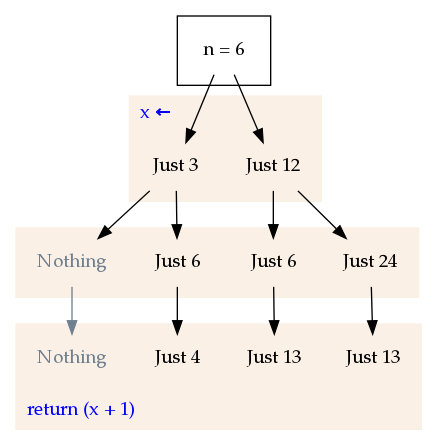
\includegraphics{/img/entries/monad-plus/halvedouble.png}
\caption{\emph{hod2PlusOne 6}, all journeys illustrated}
\end{figure}

Every complete ``journey'' is a complete path from top to bottom. You
can see that the left-left journey (the half-halve journey) fails. The
left-right journey (the halve-double journey) passes, and at the end is
given the value of \texttt{x\ +\ 1} for the \texttt{x} in that
particular journey. The other journeys work the same way!

\section{Solving real-ish problems}\label{solving-real-ish-problems}

That wasn't too bad, was it? We're actually just about ready to start
implementing our solution to the Wolf/Goat/Cabbage puzzle!

Before we end this post let's build some more familiarity with the List
monad and try out a very common practical example.

\subsection{Finding the right
combinations}\label{finding-the-right-combinations}

Here is probably the most common of all examples involving the list
monad: finding Pythagorean triples.

\begin{Shaded}
\begin{Highlighting}[]
\NormalTok{triplesUnder n }\FunctionTok{=} \KeywordTok{do}
    \NormalTok{a }\OtherTok{<-} \NormalTok{[}\DecValTok{1}\FunctionTok{..}\NormalTok{n]                     }\CommentTok{-- 1}
    \NormalTok{b }\OtherTok{<-} \NormalTok{[a}\FunctionTok{..}\NormalTok{n]                     }\CommentTok{-- 2}
    \NormalTok{c }\OtherTok{<-} \NormalTok{[b}\FunctionTok{..}\NormalTok{n]                     }\CommentTok{-- 3}
    \NormalTok{guard }\FunctionTok{$} \NormalTok{a}\FunctionTok{^}\DecValTok{2} \FunctionTok{+} \NormalTok{b}\FunctionTok{^}\DecValTok{2} \FunctionTok{==} \NormalTok{c}\FunctionTok{^}\DecValTok{2}        \CommentTok{-- 4}
    \NormalTok{return (a,b,c)                  }\CommentTok{-- 5}
\end{Highlighting}
\end{Shaded}

(\href{https://github.com/mstksg/inCode/blob/master/code-samples/monad-plus/TriplesUnder.hs}{Download
it and try it out yourself!})

\begin{enumerate}
\def\labelenumi{\arabic{enumi}.}
\tightlist
\item
  Our journey begins with picking a number between 1 and \texttt{n} and
  setting it to \texttt{a}.
\item
  Next, we pick a number between \texttt{a} and \texttt{n} and set it to
  \texttt{b}. We start from \texttt{a} because if we don't, we are
  probably going to be testing the same tuple twice.
\item
  Next, we pick a number between \texttt{b} and \texttt{n}. This is our
  hypotenuse, and of course all hypontenii are larger than either side.
\item
  Now, we mercilessly and ruthlessly end all journeys who were
  unfortunate enough to pick a non-Pythagorean combination ---
  combinations where \texttt{a\^{}2\ +\ b\^{}2} is not \texttt{c\^{}2}
\item
  For those successful journeys, we succeed with a tuple containing our
  victorious triple \texttt{(a,b,c)}.
\end{enumerate}

Let's try ``following'' this path with some arbitrary choices, looking
at arbitrary journeys for \texttt{n\ =\ 10}:

\begin{itemize}
\tightlist
\item
  We pick \texttt{a} as 2, \texttt{b} as 3, and \texttt{c} as 9. All is
  good until we get to the guard. \texttt{a\^{}2\ +\ b\^{}2} is 10,
  which is not \texttt{c\^{}2} (81), unfortunately. This
  \texttt{(2,3,10)} journey ends here.
\item
  We pick \texttt{a} as 3, \texttt{b} as 4, and \texttt{c} as 5. On the
  guard, we succeed: \texttt{a\^{}2\ +\ b\^{}2} is 25, which indeed is
  \texttt{c\^{}2}. Our journey passes the guard, and then succeeds with
  a value of \texttt{(3,4,5)}. This is indeed counted among the
  successful paths --- among the victorious!
\end{itemize}

Paths like \texttt{a\ =\ 5} and \texttt{b\ =\ 3} do not even happen.
This is because if we pick \texttt{a\ =\ 5}, then in that particular
journey, \texttt{b} can only be chosen between \texttt{5} and \texttt{n}
inclusive.

Remember, the final result is the accumulation of \textbf{all such
successful journeys}. A little bit of combinatorics will show that there
are \(\frac{1}{6} \times \frac{(n+2)!}{(n-1)!}\) possible journeys to
attempt. Only the ones that do not fail (at the guard) will make it to
the end. Remember how MonadPlus works --- one failure along the journey
means that the \emph{entire journey} is a failure.

Let's see what we get when we try it at the prompt:

\begin{Shaded}
\begin{Highlighting}[]
\NormalTok{λ}\FunctionTok{:} \NormalTok{triplesUnder }\DecValTok{10}
\NormalTok{[ ( }\DecValTok{3}\NormalTok{, }\DecValTok{4}\NormalTok{, }\DecValTok{5}\NormalTok{),( }\DecValTok{6}\NormalTok{, }\DecValTok{8}\NormalTok{,}\DecValTok{10}\NormalTok{) ]}
\NormalTok{λ}\FunctionTok{:} \NormalTok{triplesUnder }\DecValTok{25}
\NormalTok{[ ( }\DecValTok{3}\NormalTok{, }\DecValTok{4}\NormalTok{, }\DecValTok{5}\NormalTok{),( }\DecValTok{5}\NormalTok{,}\DecValTok{12}\NormalTok{,}\DecValTok{13}\NormalTok{),( }\DecValTok{6}\NormalTok{, }\DecValTok{8}\NormalTok{,}\DecValTok{10}\NormalTok{),( }\DecValTok{7}\NormalTok{,}\DecValTok{24}\NormalTok{,}\DecValTok{25}\NormalTok{)}
 \NormalTok{,( }\DecValTok{8}\NormalTok{,}\DecValTok{15}\NormalTok{,}\DecValTok{17}\NormalTok{),( }\DecValTok{9}\NormalTok{,}\DecValTok{12}\NormalTok{,}\DecValTok{15}\NormalTok{),(}\DecValTok{12}\NormalTok{,}\DecValTok{16}\NormalTok{,}\DecValTok{20}\NormalTok{),(}\DecValTok{15}\NormalTok{,}\DecValTok{20}\NormalTok{,}\DecValTok{25}\NormalTok{) ]}
\end{Highlighting}
\end{Shaded}

Perfect! You can probably quickly verify that all of these solutions are
indeed Pythagorean triples. Out of the 220 journeys undertaken by
\texttt{triplesUnder\ 10}, only two of them survived to the end to be
successful. Out of the 2925 journeys in \texttt{triplesUnder\ 25}, only
eight of them made it to the end. The rest ``died''/failed, and as a
result we do not even observe their remains. It is a cruel and
unforgiving world.

While the full diagram of \texttt{triplesUnder\ 5} has 35 branches, here
is a diagram for those branches with \(a > 2\), which has 10:

\begin{figure}[htbp]
\centering
\includegraphics{/img/entries/monad-plus/triplesunder.png}
\caption{\emph{triplesUnder 5}, all journeys (where a \textgreater{} 2)
illustrated}
\end{figure}

\section{Almost There!}\label{almost-there}

Let's do a quick review:

\begin{itemize}
\tightlist
\item
  You can really treat List exactly as if it were Maybe by using the
  general MonadPlus terms \texttt{mzero} and \texttt{return}. If you do
  this, \texttt{Nothing} is equivalent to \texttt{{[}{]}}, and
  \texttt{Just\ x} is equivalent to \texttt{{[}x{]}}. Trippy!
\item
  However, whereas Maybe is a ``deterministic'' success, for a list, a
  list of successes represents the end results of \emph{possible paths}
  to success. Chaining two ``path splits'' results in the item having to
  traverse both splits one after another.
\item
  If any of these paths meet a failure at some point in their journey,
  the entire path is a failure and doesn't show up in the list of
  successes. \emph{This} is the ``MonadPlus''ness of it all.
\item
  When you use a do block (or reason about paths), it helps to think of
  each do block as representing one specific path in a Maybe monad, with
  arbitrary choices. Your \texttt{\textless{}-} binds all represent
  \emph{one specific element}, \emph{just} like for Maybe.
\end{itemize}

The last point is particularly important and is pretty pivotal in
understanding what is coming up next. Remember that all Maybe blocks and
List blocks really essentially look \emph{exactly the same}. This
keeping-track-of-separate-paths thing is all handled behind-the scenes.

In fact you should be able to look at code like:

\begin{Shaded}
\begin{Highlighting}[]
\NormalTok{triplesUnder n }\FunctionTok{=} \KeywordTok{do}
    \NormalTok{a }\OtherTok{<-} \NormalTok{[}\DecValTok{1}\FunctionTok{..}\NormalTok{n]}
    \NormalTok{b }\OtherTok{<-} \NormalTok{[a}\FunctionTok{..}\NormalTok{n]}
    \NormalTok{c }\OtherTok{<-} \NormalTok{[b}\FunctionTok{..}\NormalTok{n]}
    \NormalTok{guard }\FunctionTok{$} \NormalTok{a}\FunctionTok{^}\DecValTok{2} \FunctionTok{+} \NormalTok{b}\FunctionTok{^}\DecValTok{2} \FunctionTok{==} \NormalTok{c}\FunctionTok{^}\DecValTok{2}
    \NormalTok{return (a,b,c)}
\end{Highlighting}
\end{Shaded}

and see that it is structurally identical to

\begin{Shaded}
\begin{Highlighting}[]
\NormalTok{triplesUnder' n }\FunctionTok{=} \KeywordTok{do}
    \NormalTok{a }\OtherTok{<-} \DataTypeTok{Just} \DecValTok{3}
    \NormalTok{b }\OtherTok{<-} \DataTypeTok{Just} \DecValTok{5}
    \NormalTok{c }\OtherTok{<-} \DataTypeTok{Just} \DecValTok{8}
    \NormalTok{guard }\FunctionTok{$} \NormalTok{a}\FunctionTok{^}\DecValTok{2} \FunctionTok{+} \NormalTok{b}\FunctionTok{^}\DecValTok{2} \FunctionTok{==} \NormalTok{c}\FunctionTok{^}\DecValTok{2}
    \NormalTok{return (a,b,c)}
\end{Highlighting}
\end{Shaded}

for any arbitrary choice of \texttt{a}, \texttt{b}, and \texttt{c},
except instead of \texttt{Just\ 3} (or \texttt{{[}3{]}}), you have
\texttt{{[}2,3,4{]}}, etc.

In fact recall that this block:

\begin{Shaded}
\begin{Highlighting}[]
\OtherTok{genericHalve ::} \DataTypeTok{MonadPlus} \NormalTok{m }\OtherTok{=>} \DataTypeTok{Int} \OtherTok{->} \NormalTok{m }\DataTypeTok{Int}
\NormalTok{genericHalve n }\FunctionTok{=} \KeywordTok{do}
    \NormalTok{guard }\FunctionTok{$} \NormalTok{even n}
    \NormalTok{return }\FunctionTok{$} \NormalTok{n }\OtherTok{`div`} \DecValTok{2}
\end{Highlighting}
\end{Shaded}

is general enough that it works for both.

Hopefully this all serves to show that \textbf{in do blocks, Lists and
Maybes are structurally identical}. You reason with them the exact same
way you do with Maybe's. In something like
\texttt{x\ \textless{}-\ Just\ 5}, \texttt{x} represents a
\textbf{single value}, the 5. In something like
\texttt{x\ \textless{}-\ {[}1,2,3{]}}, \texttt{x} \emph{also} represents
a single value --- the 1, the 2, or the 3, depending on which path you
are currently on. Then later in the block, you can refer to \texttt{x},
and \texttt{x} refers to \emph{that} one specific \texttt{x} for that
path.

\subsection{Until next time}\label{until-next-time}

So I feel like we are at all we need to know to really use the list
monad to solve a large class of logic problems (because who needs
Prolog, anyway?).

Between now and next time, think about how you would approach a logic
problem like the Wolf/Goat/Cabbage problem with the concepts of
MonadPlus? What would \texttt{mzero}/fail be useful for? What would the
idea of a success be useful for, and what would the idea of ``multiple
paths to success'' in a journey even mean? What is the journey?

Until next!

\end{document}
